\chapter{TCP: segmenti, numeri di sequenza e ritrasmissione}

% ══════════════════════════════════════════════════════════════
\section{TCP a confronto con UDP}
% ══════════════════════════════════════════════════════════════

Tutti i meccanismi sono pronti: checksum, numeri di sequenza, conferme, timer, una finestra. Ora ricevono un header.
TCP conferma in modo cumulativo, come Go-Back-N, e tiene ciò che arriva in anticipo, come Selective Repeat; e una
decisione attraversa tutto il capitolo: \textbf{i numeri contano byte, non pacchetti}.

Rispetto a UDP, TCP è:

\begin{itemize}
    \item \textbf{orientato alla connessione}: prima della trasmissione c'è una fase di \emph{handshake} che
          assicura che i due processi (mittente e ricevente) siano ``collegati'';
    \item \textbf{affidabile}: implementa rilevazione degli errori, ritrasmissioni, conferme, timer e numeri di sequenza;
    \item \textbf{attento al flusso e alla congestione}: regola la velocità di trasmissione in base alle capacità
          del ricevente (flusso) e allo stato della rete (congestione).
\end{itemize}

\dfn{Proprietà della connessione TCP}{
    \begin{itemize}
      \item \textbf{Full-duplex}: se l'host A è connesso con B, anche B è connesso con A, e i dati possono
            scorrere contemporaneamente nelle due direzioni.
      \item \textbf{Punto-punto}: un solo mittente e un solo ricevente. Non è possibile trasferire dati da un
            mittente a molti riceventi con una sola connessione (UDP, invece, permette il \emph{multicasting}).
      \item \textbf{Orientato al flusso di byte} (\emph{stream}): più segmenti TCP possono far parte di un unico
            flusso ordinato di dati, mentre i datagrammi UDP sono sostanzialmente indipendenti tra loro.
            L'applicazione consegna byte, non messaggi, e dove cadono i confini dei segmenti lo decide TCP.
    \end{itemize}
}

\subsection{Una connessione senza niente in mezzo}

\dfn{Connessione logica}{
    I due moduli di trasporto si comportano come se un canale affidabile li unisse direttamente. Sotto, i segmenti
    attraversano una rete che sa solo instradare.
}

\begin{itemize}
    \item \textbf{Non è un circuito}: non si riserva capacità, e dentro la rete non si mette da parte niente per la
          connessione.
    \item Buffer, variabili e timer esistono \textbf{nei due sistemi terminali} e da nessun'altra parte.
    \item I router vedono datagrammi, non connessioni: inoltrano il segmento senza leggere un byte del suo header.
    \item È per questo che l'affidabilità si costruisce qui: il livello di rete è occupato a decidere \emph{dove} va un
          pacchetto, non \emph{se} è arrivato.
\end{itemize}

% ══════════════════════════════════════════════════════════════
\section{I buffer TCP}
% ══════════════════════════════════════════════════════════════

In una connessione TCP l'invio e la ricezione si basano sui \textbf{buffer}. I buffer permettono di
disaccoppiare, almeno in parte, i tempi di trasmissione dai ritardi dell'applicazione, dai ritardi del
sistema operativo nel multiplexing e demultiplexing, e dalle oscillazioni delle prestazioni della rete.
Inoltre la velocità di trasmissione è limitata: i messaggi lunghi vengono spezzati in segmenti, che si
accumulano nei buffer prima di essere spediti (lato mittente) o riassemblati (lato ricevente).

\begin{figure}[H]
\centering
\begin{tikzpicture}[every node/.style={font=\footnotesize\sffamily}]
  \node[draw, circle, fill=lapp!60, minimum size=1cm] (pa) at (0,2) {A};
  \node[above=1pt of pa] {processo mittente};
  \node[field, fill=ltra!50, minimum width=0.6cm] (sk1) at (0,0.9) {};
  \node[left=2pt of sk1] {socket};
  \node[draw, fill=llink!50, minimum width=2.8cm, minimum height=0.8cm] (sb) at (0,-0.3) {};
  \foreach \x in {-1.1,-0.6,-0.1} \fill[netblue!60] (\x,-0.55) rectangle ++(0.4,0.5);
  \node[below=1pt of sb] {buffer di invio};
  \node[draw, circle, fill=lapp!60, minimum size=1cm] (pb) at (9,2) {B};
  \node[above=1pt of pb] {processo ricevente};
  \node[field, fill=ltra!50, minimum width=0.6cm] (sk2) at (9,0.9) {};
  \node[right=2pt of sk2] {socket};
  \node[draw, fill=llink!50, minimum width=2.8cm, minimum height=0.8cm] (rb) at (9,-0.3) {};
  \foreach \x in {8.0,8.5} \fill[netblue!60] (\x,-0.55) rectangle ++(0.4,0.5);
  \node[below=1pt of rb] {buffer di ricezione};
  \draw[-{Stealth}, thick] (pa) -- (sk1); \draw[-{Stealth}, thick] (sk1) -- (sb);
  \draw[-{Stealth}, thick] (rb) -- (sk2); \draw[-{Stealth}, thick] (sk2) -- (pb);
  \foreach \x in {3.4,4.5,5.6} { \fill[ltra] (\x,-0.5) rectangle ++(0.3,0.4); \fill[netblue!50] (\x+0.3,-0.5) rectangle ++(0.5,0.4); \draw (\x,-0.5) rectangle ++(0.8,0.4); }
  \draw[-{Stealth}, very thick, netblue] (sb.east) -- node[below=10pt] {segmenti} (rb.west);
\end{tikzpicture}
\caption{Ogni lato di una connessione TCP ha un buffer di invio e uno di ricezione.}
\end{figure}

\begin{itemize}
    \item \textbf{In invio}: \texttt{write} non trasmette; \textbf{copia} i byte nel buffer di invio, e TCP li spedisce da lì
          quando gli conviene, creando i segmenti e passandoli al livello di rete.
    \item \textbf{In ricezione}: \texttt{read} non riceve; prende ciò che è già nel buffer di ricezione, messo lì da
          segmenti arrivati prima.
    \item I due buffer assorbono la differenza fra quanto velocemente scrive l'applicazione, quanto velocemente si muove la
          rete e quanto velocemente legge l'altro lato. Ogni estremo ne ha uno di ciascun tipo, perché ogni estremo sia
          invia sia riceve.
\end{itemize}

Ecco perché, nella parte sulla programmazione, una \texttt{write} di 1000 byte poteva arrivare in tre \texttt{read}:
le due chiamate non toccano la rete, toccano due buffer diversi.

% ══════════════════════════════════════════════════════════════
\section{La Maximum Segment Size (MSS)}
% ══════════════════════════════════════════════════════════════

\dfn{MSS e MTU}{
    La quantità di dati applicativi in un segmento è limitata dalla \textbf{Maximum Segment Size} (MSS):
    $$\text{MSS} + 40 = \text{MTU}$$
    dove la \textbf{Maximum Transmission Unit} (MTU) è la lunghezza massima di un frame accettata dal livello
    di collegamento (in Ethernet \textbf{1500 byte}), e 40 è la somma tipica degli header TCP e IP (20 + 20 byte).
}

\begin{figure}[H]
\centering
\begin{tikzpicture}[every node/.style={font=\scriptsize\sffamily}]
  \node[field, fill=lnet, minimum width=2.2cm] (ip) at (0,0) {header IP: 20};
  \node[field, fill=ltra, minimum width=2.2cm, right=0pt of ip] (tcp) {header TCP: 20};
  \node[field, fill=lapp, minimum width=8cm, right=0pt of tcp] (d) {dati applicativi: al massimo MSS = 1460 byte};
  \draw[decorate, decoration={brace, amplitude=5pt}] ([yshift=2pt]ip.north west) -- ([yshift=2pt]d.north east) node[midway, above=6pt] {MTU di Ethernet = 1500 byte (payload del frame)};
\end{tikzpicture}
\caption{Con MTU di 1500 byte e header da 20 + 20 byte, la MSS tipica è di 1460 byte.}
\end{figure}

La MSS è la quantità di \textbf{dati} in un segmento, non la dimensione del segmento. E un'immagine da tre megabyte non è
un messaggio: sono duemila segmenti, e l'applicazione non viene mai a sapere dove sono caduti i tagli.

% ══════════════════════════════════════════════════════════════
\section{Il segmento TCP}
% ══════════════════════════════════════════════════════════════

\begin{figure}[H]
\centering
\begin{tikzpicture}[every node/.style={font=\scriptsize\sffamily}, x=0.45cm, y=0.62cm]
  \def\row#1#2#3#4{\node[field, fill=#4, minimum width=#2*0.45cm, minimum height=0.62cm, anchor=north west] at (#1,-#3) {};}
  % riga 1
  \node[field, fill=ltra, minimum width=7.2cm, minimum height=0.62cm, anchor=north west] at (0,0) {porta sorgente (16)};
  \node[field, fill=ltra, minimum width=7.2cm, minimum height=0.62cm, anchor=north west] at (16,0) {porta destinazione (16)};
  \node[field, fill=lapp!60, minimum width=14.4cm, minimum height=0.62cm, anchor=north west] at (0,-1) {numero di sequenza (32)};
  \node[field, fill=lapp!60, minimum width=14.4cm, minimum height=0.62cm, anchor=north west] at (0,-2) {numero di acknowledgment (32)};
  \node[field, fill=lnet!50, minimum width=1.8cm, minimum height=1.1cm, anchor=north west, align=center] at (0,-3) {lungh.\\header};
  \node[field, fill=lphy, minimum width=1.8cm, minimum height=1.1cm, anchor=north west, align=center] at (4,-3) {non\\usato};
  \foreach \f [count=\i from 0] in {CWR,ECE,URG,ACK,PSH,RST,SYN,FIN}
    \node[field, fill=netred!20, minimum width=0.45cm, minimum height=1.1cm, anchor=north west] at (8+\i,-3) {\rotatebox{90}{\f}};
  \node[field, fill=llink, minimum width=7.2cm, minimum height=1.1cm, anchor=north west] at (16,-3) {finestra di ricezione (16)};
  \node[field, fill=ltra!50, minimum width=7.2cm, minimum height=0.62cm, anchor=north west] at (0,-4.77) {checksum (16)};
  \node[field, fill=ltra!50, minimum width=7.2cm, minimum height=0.62cm, anchor=north west] at (16,-4.77) {puntatore ai dati urgenti (16)};
  \node[field, fill=lphy!60, minimum width=14.4cm, minimum height=0.62cm, anchor=north west] at (0,-5.77) {opzioni (lunghezza variabile)};
  \node[field, fill=cloudbg, minimum width=14.4cm, minimum height=1.3cm, anchor=north west] at (0,-6.77) {dati (al massimo MSS byte)};
  \draw[{Stealth}-{Stealth}] (0,0.5) -- node[above] {32 bit} (32,0.5);
  \draw[decorate, decoration={brace, amplitude=5pt}] (32.4,0) -- (32.4,-6.77) node[midway, right=6pt, align=left] {header:\\20 byte\\+ opzioni};
\end{tikzpicture}
\caption{La struttura del segmento TCP.}
\end{figure}

Il segmento TCP è fatto di un header e di un campo dati, che contiene al massimo MSS byte di dati
applicativi. I campi dell'header:

\begin{itemize}
    \item \textbf{porta sorgente} e \textbf{porta destinazione} (16 bit ciascuna): per multiplexing e demultiplexing;
    \item \textbf{numero di sequenza} (32 bit) e \textbf{numero di acknowledgment} (32 bit): per il trasferimento affidabile;
    \item \textbf{finestra di ricezione} (\emph{receive window}, 16 bit): il numero di byte che il ricevente è
          disposto ad accettare (serve al controllo di flusso);
    \item \textbf{lunghezza dell'header} (4 bit): il numero di parole da 32 bit dell'header. L'header TCP ha
          lunghezza variabile per via delle opzioni (tipicamente 20 byte senza opzioni);
    \item \textbf{opzioni} (lunghezza variabile): per processi facoltativi come la negoziazione della MSS o i timestamp;
    \item \textbf{flag}:
    \begin{itemize}
      \item \textbf{ACK}: il segmento contiene una conferma (il campo acknowledgment è valido);
      \item \textbf{RST}, \textbf{SYN}, \textbf{FIN}: apertura e chiusura della connessione;
      \item \textbf{CWR} e \textbf{ECE}: notifica esplicita della congestione (ECN), in cui è la rete a dire ai due estremi
            che è congestionata, invece di limitarsi a scartare;
      \item \textbf{PSH}: chiede al ricevente di passare subito i dati all'applicazione;
      \item \textbf{URG}: il segmento contiene dati ``urgenti'', e il puntatore dice dove finiscono.
    \end{itemize}
    Otto flag, con quattro bit inutilizzati accanto; gli ultimi due (PSH e URG) in pratica non si usano;
    \item \textbf{checksum} (16 bit): controllo di integrità, come in UDP;
    \item \textbf{puntatore ai dati urgenti} (16 bit): la posizione dell'ultimo byte dei dati urgenti (raro).
\end{itemize}

% ══════════════════════════════════════════════════════════════
\section{Numeri di sequenza e di acknowledgment}
% ══════════════════════════════════════════════════════════════

I numeri di sequenza non servono solo al trasferimento affidabile, ma anche a gestire la
\textbf{segmentazione}: un flusso di dati grande va spezzato in ``pezzi'' in base alla MSS, e ogni pezzo va in un
segmento. Numeri di sequenza e di acknowledgment sono strettamente legati.

TCP è un protocollo di trasporto generico: non sa nulla dei dati che trasporta. Per TCP i dati sono
solo un \textbf{flusso ordinato di byte}, e i numeri contano \textbf{byte}, non segmenti.

\dfn{Numero di sequenza e numero di acknowledgment}{
    \begin{itemize}
      \item Il \textbf{numero di sequenza} di un segmento è la posizione, nel flusso di byte, del \textbf{primo
            byte di dati} contenuto nel segmento.
      \item Il \textbf{numero di acknowledgment} è il numero di sequenza del \textbf{prossimo byte atteso} dal
            ricevente. Gli ACK di TCP sono \textbf{cumulativi}: ACK $n$ conferma tutti i byte fino a $n-1$.
    \end{itemize}
}

\begin{figure}[H]
\centering
\begin{tikzpicture}[every node/.style={font=\scriptsize\sffamily}]
  \draw[thick] (0,0) rectangle (14,0.7);
  \fill[lapp!70] (0,0) rectangle (2,0.7); \fill[ltra!70] (2,0) rectangle (4,0.7); \fill[lnet!70] (4,0) rectangle (6,0.7);
  \foreach \x in {2,4,6,8,10,12} \draw (\x,0) -- (\x,0.7);
  \node at (1,0.35) {segmento 1}; \node at (3,0.35) {segmento 2}; \node at (5,0.35) {segmento 3}; \node at (9,0.35) {\dots};
  \foreach \x/\n in {0/0, 2/1000, 4/2000, 6/3000} \node[below] at (\x,0) {\n};
  \node[below] at (13.9,0) {499\,999};
  \draw[{Stealth}-, thick, netred] (0,0.8) -- ++(0,0.6) node[above, text=netred] {seq = 0};
  \draw[{Stealth}-, thick, netred] (2,0.8) -- ++(0,0.6) node[above, text=netred] {seq = 1000};
  \draw[{Stealth}-, thick, netred] (4,0.8) -- ++(0,0.6) node[above, text=netred] {seq = 2000};
  \draw[decorate, decoration={brace, amplitude=5pt, mirror}] (0,-0.5) -- (2,-0.5) node[midway, below=6pt] {MSS = 1000 byte};
  \node[anchor=west] at (14.1,0.35) {file da 500\,000 byte};
\end{tikzpicture}
\caption{Un file di 500\,000 byte con MSS di 1000 byte: 500 segmenti, con numeri di sequenza 0, 1000, 2000, \dots}
\end{figure}

\begin{esempio}{Un file di 500 kB}
Un flusso di 500\,000 byte con MSS di 1000 byte diventa \textbf{500 segmenti}: il primo ha numero di
sequenza 0, il secondo 1000, il terzo 2000, e così via. Trascurando per semplicità lo scambio iniziale
(nella realtà il primo numero di sequenza è scelto a caso), dall'host A all'host B:
\begin{itemize}
    \item B riceve il primo segmento, con i byte da 0 a 999;
    \item B conferma con numero di acknowledgment \textbf{1000}: il prossimo byte che si aspetta;
    \item B riceve il secondo segmento, byte da 1000 a 1999, e conferma con ACK \textbf{2000}; e così via.
\end{itemize}
\end{esempio}

\warning{ACK $n$ non conferma il byte $n$}{
    L'errore più comune: ACK = 1000 \textbf{non} significa ``ho ricevuto il byte 1000'', ma ``ho ricevuto tutto
    fino al 999, mandami dal 1000 in poi''. Il numero esiste anche prima di qualsiasi dato: appena la connessione è aperta,
    B aspetta già un byte preciso.
}

\subsection{Conferme cumulative, e un segmento in anticipo}

\begin{esempio}{Un buco nel flusso}
A ha ricevuto da B i byte 0--535, e poi un segmento con i byte 900--1000. I byte 536--899 non sono mai arrivati. A
conferma \textbf{536}.
\end{esempio}

\begin{itemize}
    \item Una conferma dice «tutto ciò che sta sotto questo numero è arrivato», e \textbf{niente} su ciò che sta sopra.
    \item Quindi una conferma copre un numero qualsiasi di segmenti, e perderne una non costa niente purché ne passi una
          successiva.
    \item Non c'è modo di riferire i cento byte che A sta tenendo: l'header ha un numero solo, e il buco viene prima.
    \item Quel numero unico è ciò che rende economico il mittente, e costoso un segmento mancante.
\end{itemize}

E i byte 900--1000, arrivati in anticipo: tenerli o buttarli? \textbf{Le RFC non lo decidono}: entrambi i comportamenti
sono corretti, e la scelta è lasciata a chi scrive l'implementazione. Buttandoli il ricevente resta semplice e il
mittente paga rimandandoli; tenendoli i byte aspettano che il buco si riempia, e la rete trasporta ogni byte una volta.
\textbf{Tutte le implementazioni in uso li tengono}, ed è per questo che una perdita costa una ritrasmissione e non una
finestra intera.

\subsection{Il caso full-duplex}

TCP è full-duplex: se A e B comunicano ci sono \textbf{due flussi} di dati da rendere affidabili, da A a B
e da B ad A. Si usano numeri di sequenza e di acknowledgment \textbf{contemporaneamente}:

\begin{itemize}
    \item i segmenti inviati da A hanno numeri di \textbf{sequenza} relativi al flusso A$\rightarrow$B e numeri di
          \textbf{acknowledgment} relativi al flusso B$\rightarrow$A;
    \item i segmenti inviati da B hanno numeri di sequenza relativi al flusso B$\rightarrow$A e numeri di
          acknowledgment relativi al flusso A$\rightarrow$B.
\end{itemize}

Un segmento può quindi portare \textbf{insieme dati e conferma} (si dice che l'ACK viaggia ``a cavalluccio'',
\emph{piggybacking}), con il flag ACK a 1.

\begin{esempio}{L'eco di un carattere (Telnet)}
\begin{center}
\begin{tikzpicture}[yscale=0.9, every node/.style={font=\scriptsize\sffamily}]
  \timeline{a}{0}{Host A}{5}
  \timeline{b}{7}{Host B}{5}
  \draw[msg, netgreen, very thick] (0,-0.5) -- node[above, sloped] {Seq=42, ACK=79, dati=`C'} (7,-1.5);
  \node[anchor=east, text width=2.6cm, align=right] at (-0.2,-0.5) {l'utente digita `C'};
  \draw[msg, netred, very thick] (7,-2.0) -- node[above, sloped] {Seq=79, ACK=43, dati=`C'} (0,-3.0);
  \node[anchor=west, text width=2.8cm, align=left] at (7.2,-2.0) {B conferma la `C' e la rimanda indietro (eco)};
  \draw[msg, netgreen, very thick] (0,-3.5) -- node[above, sloped] {Seq=43, ACK=80} (7,-4.5);
  \node[anchor=east, text width=2.6cm, align=right] at (-0.2,-3.5) {A conferma l'eco (ACK puro, senza dati)};
\end{tikzpicture}
\end{center}
Due messaggi da un solo byte: A invia la `C', che B rimanda indietro. In verde le informazioni sul flusso
A$\rightarrow$B, in rosso quelle sul flusso B$\rightarrow$A.
\begin{enumerate}
    \item \textbf{Da A a B}: il numero di sequenza è la posizione del byte trasmesso (42); l'ACK è il prossimo byte
          atteso sul flusso B$\rightarrow$A (79).
    \item \textbf{Da B ad A}: l'ACK è il prossimo byte atteso sul flusso A$\rightarrow$B, cioè $42 + 1$ byte $= 43$;
          il numero di sequenza è la posizione del byte che B trasmette (79), proprio quello che A aspettava.
    \item \textbf{Da A a B}: un ACK puro, con numero di sequenza 43 (come atteso da B) e ACK $79 + 1 = 80$.
\end{enumerate}
In ogni scambio vale: \textbf{ACK ricevuto = Seq inviato + byte inviati}, e \textbf{Seq inviato = ACK ricevuto}.
I due flussi partono da 42 e 79, concordati all'apertura della connessione, e non da zero.
\end{esempio}

\warning{Anche un segmento senza dati ha un numero di sequenza}{
    Il terzo segmento non porta niente. Che cosa ci fa \texttt{Seq=43}? Il campo è nell'header che lo si usi o no, quindi
    dice dove comincerebbe A se avesse qualcosa da inviare. \textbf{Non consuma alcun byte}: il prossimo segmento di A
    porterà di nuovo 43.
    \begin{itemize}
        \item Un ACK puro non fa avanzare il flusso, e ciò che B aspetta non si muove: sempre il byte 43.
        \item Quindi nessuno lo conferma: non c'è niente da confermare, e per lui non parte nessun timer.
        \item Se si perde non si ritrasmette niente: la prossima conferma di A porterà la stessa informazione, o di più.
    \end{itemize}
}

\subsection{Da dove parte la numerazione}

In tutti gli esempi il primo byte era numerato 0. In una connessione reale \textbf{non lo è mai}.
\begin{itemize}
    \item Ciascun lato sceglie a caso il proprio \textbf{numero di sequenza iniziale} (ISN) e lo comunica all'altro durante
          l'apertura della connessione.
    \item Il motivo è quello visto con il riuso dei numeri di sequenza: un segmento di una connessione precedente può essere
          ancora vivo nella rete.
    \item Stessi due host, stesse due porte, numerazione da zero ogni volta: una vecchia copia verrebbe accettata come
          dato attuale.
    \item Un inizio casuale non lo rende impossibile, lo rende \textbf{improbabile}, ed è il massimo che il protocollo può
          fare.
\end{itemize}

% ══════════════════════════════════════════════════════════════
\section{Il mittente TCP in tre eventi}
% ══════════════════════════════════════════════════════════════

\begin{table}[H]
\centering
\begin{tabular}{p{0.3\textwidth} p{0.62\textwidth}}
\toprule
\textbf{Evento} & \textbf{Che cosa fa il mittente} \\
\midrule
Arrivano dati dall'applicazione &
Costruisce un segmento con numero di sequenza \texttt{NextSeqNum}, avvia il timer se non è già in corsa, lo passa a IP e
fa avanzare \texttt{NextSeqNum} del numero di byte inviati. \\
Il timer scade &
Ritrasmette il segmento non confermato con il numero di sequenza più piccolo, e riavvia il timer. \\
Arriva una conferma $y$ &
Se $y > \texttt{SendBase}$, porta \texttt{SendBase} a $y$, e riavvia il timer se resta qualcosa di non confermato. \\
\bottomrule
\end{tabular}
\caption{Due variabili contengono l'intero mittente: \texttt{SendBase}, il byte più vecchio non ancora confermato, e
         \texttt{NextSeqNum}, il prossimo che partirà.}
\end{table}

\subsection{Un timer, non uno per segmento}

\begin{itemize}
    \item Un timer per ogni segmento in sospeso è il progetto naturale, ed è ciò che chiede Selective Repeat.
    \item TCP ne tiene \textbf{uno}, legato al segmento più vecchio non confermato, quello a cui punta \texttt{SendBase}.
    \item Quando scatta riparte \textbf{solo quel segmento}, per quanti altri ce ne siano in volo senza risposta: un mittente
          con dieci segmenti in sospeso ne ritrasmette uno, e lascia che le conferme cumulative sistemino il resto.
    \item Il motivo è il costo: una scadenza da seguire invece di una per segmento, su una macchina che può avere migliaia
          di connessioni.
\end{itemize}

% ══════════════════════════════════════════════════════════════
\section{Il timeout di ritrasmissione}
% ══════════════════════════════════════════════════════════════

Il trasferimento affidabile di TCP usa ampiamente i timer. Nella trasmissione TCP con pipelining
l'approccio di base è ritrasmettere un segmento \textbf{solo se il suo ACK non arriva prima del timeout}.
La stima del timeout è quindi critica:

\begin{itemize}
    \item \textbf{troppo lungo}: ogni perdita si paga con una lunga attesa a vuoto, e il trasferimento si ferma finché il
          timer corre;
    \item \textbf{troppo breve}: segmenti soltanto lenti vengono dichiarati persi, e la rete trasporta copie che nessuno
          aveva chiesto. Il caso estremo lo conosciamo: con un timeout più corto dell'andata e ritorno si ritrasmette tutto,
          senza perdere niente.
\end{itemize}
Il timeout deve quindi essere più grande dell'RTT, e l'RTT non è una costante, e nessuno dice al mittente quanto vale.

\begin{figure}[H]
\centering
\begin{tikzpicture}[yscale=0.75, every node/.style={font=\scriptsize\sffamily}]
  \begin{scope}
    \node[font=\footnotesize\bfseries\sffamily] at (1.6,1.2) {(a) ACK perso};
    \timeline{a}{0}{A}{6}
    \timeline{b}{3.2}{B}{6}
    \draw[msg] (0,-0.3) -- node[above, sloped] {Seq=92, 8 byte} (3.2,-1.1);
    \draw[msglost] (3.2,-1.3) -- (1.7,-1.7); \node[text=netred] at (1.4,-1.35) {ACK=100};
    \draw[netorange, thick] (-0.25,-0.3) -- (-0.25,-2.9); \node[text=netorange, rotate=90] at (-0.5,-1.6) {timeout};
    \draw[msg] (0,-2.9) -- node[above, sloped] {Seq=92, 8 byte} (3.2,-3.7);
    \draw[msg, netgreen] (3.2,-3.9) -- node[above, sloped] {ACK=100} (0,-4.7);
  \end{scope}
  \begin{scope}[xshift=5.2cm]
    \node[font=\footnotesize\bfseries\sffamily] at (1.6,1.2) {(b) timeout prematuro};
    \timeline{a}{0}{A}{6}
    \timeline{b}{3.2}{B}{6}
    \draw[msg] (0,-0.3) -- node[above, sloped] {Seq=92, 8 byte} (3.2,-1.1);
    \draw[msg] (0,-0.6) -- node[below, sloped] {Seq=100, 20 byte} (3.2,-1.4);
    \draw[msg, netgreen] (3.2,-1.6) -- node[above, sloped, pos=0.3] {ACK=100} (0,-2.9);
    \draw[msg, netgreen] (3.2,-1.9) -- node[below, sloped, pos=0.7] {ACK=120} (0,-3.2);
    \draw[netorange, thick] (-0.25,-0.3) -- (-0.25,-2.5); \node[text=netorange, rotate=90] at (-0.5,-1.4) {timeout};
    \draw[msg, netred] (0,-2.5) -- node[above, sloped, pos=0.7] {Seq=92 (inutile)} (3.2,-3.5);
    \draw[msg, netgreen] (3.2,-3.7) -- node[above, sloped] {ACK=120} (0,-4.5);
  \end{scope}
  \begin{scope}[xshift=10.4cm]
    \node[font=\footnotesize\bfseries\sffamily] at (1.6,1.2) {(c) ACK cumulativo};
    \timeline{a}{0}{A}{6}
    \timeline{b}{3.2}{B}{6}
    \draw[msg] (0,-0.3) -- node[above, sloped] {Seq=92, 8 byte} (3.2,-1.1);
    \draw[msg] (0,-0.6) -- node[below, sloped] {Seq=100, 20 byte} (3.2,-1.4);
    \draw[msglost] (3.2,-1.6) -- (1.9,-2.0); \node[text=netred] at (1.5,-1.65) {ACK=100};
    \draw[msg, netgreen] (3.2,-2.2) -- node[above, sloped] {ACK=120} (0,-3.0);
    \node[text width=3cm, align=center] at (1.6,-4.1) {nessuna ritrasmissione: ACK=120 conferma anche i byte 92--99};
  \end{scope}
\end{tikzpicture}
\caption{Tre scenari di ritrasmissione TCP. Nel terzo una conferma si è persa e nulla è stato inviato due volte: ACK=120
         dice che tutto ciò che sta sotto 120 è arrivato, copre entrambi i segmenti, e \texttt{SendBase} salta subito a
         120 fermando il timer.}
\end{figure}

\subsection{Raddoppiare il timeout}

\begin{itemize}
    \item Quando il timer scade, TCP ritrasmette e imposta il timeout successivo al \textbf{doppio} dell'intervallo appena
          trascorso: tre quarti di secondo diventano 1,5, poi 3, poi 6. Le attese crescono esponenzialmente finché non torna
          niente.
    \item Nel frattempo la stima non si usa: torna appena arriva una conferma e il timer riparte normalmente.
    \item Un timeout di solito significa congestione, e ritrasmettere più forte in una rete congestionata la peggiora.
          Quindi il mittente \textbf{si ritira}: è una forma rudimentale di controllo di congestione, e la stessa idea
          tornerà quando le stazioni collidono su un collegamento condiviso.
\end{itemize}

% ══════════════════════════════════════════════════════════════
\section{La stima dell'RTT}
% ══════════════════════════════════════════════════════════════

Per fissare il timeout serve una stima del \textbf{round-trip time}: il timeout (quanto aspettare l'ACK di un
segmento) deve essere maggiore dell'RTT, altrimenti si ritrasmette inutilmente.

\dfn{SampleRTT}{
    Il tempo fra la consegna di un segmento a IP e l'arrivo di una conferma che lo copre. Una misura, per un segmento.
}

\begin{itemize}
    \item TCP misura un segmento alla volta, non tutti: più o meno un nuovo campione per andata e ritorno.
    \item I campioni si muovono, e di molto: le code dei router si riempiono e si svuotano, e l'host all'altro capo ha un
          carico suo.
    \item Un singolo campione è quindi una cattiva stima dell'andata e ritorno, e una base pessima per una scadenza.
    \item E i segmenti ritrasmessi non vengono \textbf{mai} campionati.
\end{itemize}

\warning{A quale trasmissione risponde quella conferma?}{
    Un segmento parte, il timer scatta, riparte, e poi arriva una conferma. Porta un numero di byte, non un istante: è
    identica sia che risponda alla prima copia sia alla seconda, e il mittente \textbf{non può saperlo}.
    \begin{itemize}
        \item Misurando dalla prima trasmissione, il campione è troppo lungo se la conferma risponde in realtà alla
              seconda.
        \item Misurando dalla seconda, è troppo corto se la prima copia era arrivata e la sua conferma era solo lenta.
        \item Un campione corto accorcia il timeout, che produce più ritrasmissioni premature, che producono più campioni
              corti.
    \end{itemize}
    La regola (di Karn) taglia il ciclo prima che cominci: \textbf{mai campionare un segmento ritrasmesso}.
}

\dfn{EstimatedRTT}{
    Poiché i campioni oscillano (congestione, carico del ricevente, \dots), la stima è una \textbf{media mobile
    esponenziale pesata} (EWMA, \emph{Exponential Weighted Moving Average}):
    $$\text{EstimatedRTT} = (1-\alpha)\cdot\text{EstimatedRTT} + \alpha\cdot\text{SampleRTT}$$
    con $\alpha$ tipicamente $0{,}125 = 1/8$.
}

\begin{itemize}
    \item Ogni nuovo campione tira la stima di un ottavo verso di sé: una misura strana non può trascinarla lontano.
    \item Il peso di un campione vecchio si riduce di $7/8$ a ogni aggiornamento, esponenzialmente, da cui il nome.
    \item Quindi la media \textbf{dimentica}: ciò che faceva il percorso un minuto fa ora non conta quasi niente, ed è
          proprio lo scopo.
    \item Non si conserva alcuna storia: una variabile, e due operazioni per conferma.
\end{itemize}

\begin{figure}[H]
    \centering
    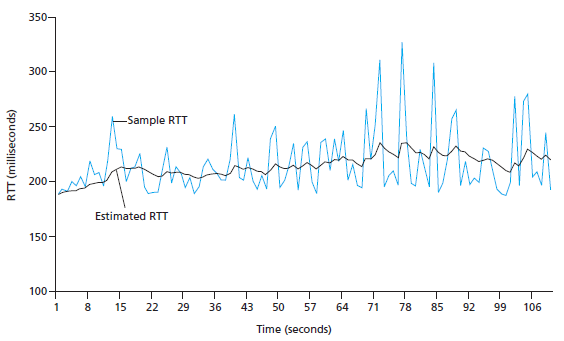
\includegraphics[width=0.62\linewidth]{cap10/rtt_campioni.png}
    \caption{Campioni di RTT (azzurro) e stima EWMA (nero) in una connessione reale tra Stati Uniti e Francia.}
\end{figure}

\dfn{DevRTT}{
    Si stima anche la \textbf{variabilità} dell'RTT, come media mobile della differenza tra campione e stima:
    $$\text{DevRTT} = (1-\beta)\cdot\text{DevRTT} + \beta\cdot|\,\text{SampleRTT} - \text{EstimatedRTT}\,|$$
    con $\beta$ tipicamente $0{,}25 = 1/4$.
}

\subsection{Il timeout}

\dfn{TimeoutInterval}{
    $$\text{TimeoutInterval} = \text{EstimatedRTT} + 4\cdot\text{DevRTT}$$
    La stima fissa il \textbf{minimo}: sotto, le conferme arriverebbero dopo che il timer è già scattato. La deviazione
    fornisce il \textbf{margine}, ampio quando il percorso è irregolare, stretto quando è stabile. Così il timeout segue
    un collegamento che comincia a comportarsi male senza che nessuno debba scegliere un numero. Prima del primo campione
    non c'è niente da cui calcolare, quindi il valore iniziale è di \textbf{1 secondo}; e dopo una ritrasmissione la
    formula si mette da parte e l'intervallo raddoppia, finché non torna qualcosa.
}

\begin{esempio}{Aggiornare stima e timeout}
Siano $\text{EstimatedRTT} = 100$ ms, $\text{DevRTT} = 10$ ms, e arrivi un campione $\text{SampleRTT} = 140$ ms.
\begin{align*}
\text{EstimatedRTT} &= 0{,}875 \cdot 100 + 0{,}125 \cdot 140 = 87{,}5 + 17{,}5 = 105 \text{ ms}\\
\text{DevRTT} &= 0{,}75 \cdot 10 + 0{,}25 \cdot |140 - 105| = 7{,}5 + 8{,}75 = 16{,}25 \text{ ms}\\
\text{TimeoutInterval} &= 105 + 4 \cdot 16{,}25 = 170 \text{ ms}
\end{align*}
\end{esempio}

\info{Due dettagli pratici}{
    \begin{itemize}
      \item Nello standard (RFC 6298) \texttt{DevRTT} viene aggiornata \emph{prima} di \texttt{EstimatedRTT},
            usando il valore vecchio della stima; molti testi, come le trasparenze, le presentano nell'ordine
            inverso. Negli esercizi seguite l'ordine indicato dal testo.
      \item Quando scade un timeout, TCP ritrasmette e \textbf{raddoppia} il timeout, invece di ricalcolarlo: se c'è
            congestione, non ha senso ritrasmettere sempre più in fretta.
    \end{itemize}
}

% ══════════════════════════════════════════════════════════════
\section{Fast retransmit}
% ══════════════════════════════════════════════════════════════

La ritrasmissione dopo il timeout funziona, ma il timeout può essere relativamente lungo. Prima di vedere come
accorciarlo, bisogna sapere quando il ricevente invia una conferma.

\begin{table}[H]
\centering
\begin{tabular}{p{0.44\textwidth} p{0.48\textwidth}}
\toprule
\textbf{Che cosa arriva} & \textbf{Che cosa fa il ricevente} \\
\midrule
Segmento in ordine, e tutto ciò che lo precede è già confermato &
Aspetta fino a 500 ms il successivo; se non arriva, conferma. \\
Segmento in ordine, con un segmento precedente ancora da confermare &
Conferma entrambi insieme, con un numero solo. \\
Segmento fuori ordine, con numero più alto dell'atteso: un buco &
Conferma \textbf{subito}, ripetendo il numero del fondo del buco. \\
Un segmento che riempie il buco &
Conferma subito, fino alla fine di ciò che ora è contiguo. \\
\bottomrule
\end{tabular}
\caption{Quando il ricevente TCP invia una conferma. La prima riga è la \textbf{conferma ritardata}
         (\emph{delayed ACK}): due segmenti, una risposta. La terza è da dove vengono i duplicati.}
\end{table}

\subsection{Le conferme duplicate}

\begin{itemize}
    \item Una conferma duplicata ripete un numero che il mittente aveva già: presa da sola non porta alcuna informazione
          nuova.
    \item Ma è stata inviata per una ragione: al ricevente è arrivato qualcosa, e non era ciò che serviva al buco.
    \item Ogni duplicato è quindi la prova che i segmenti dopo quello mancante stanno passando: il percorso funziona, un
          segmento no.
    \item Un mittente che qui aspetta il suo timer sta aspettando una scadenza di cui ha già la risposta.
    \item TCP non ha conferme negative: un numero ripetuto è la cosa più vicina, e non costa un nuovo tipo di pacchetto.
\end{itemize}

\dfn{Fast retransmit}{
    Con la \textbf{ritrasmissione veloce} il ricevente segnala al mittente che un segmento potrebbe essere
    perso inviando \textbf{ACK duplicati}.
    \begin{itemize}
      \item Se il ricevente riceve un segmento con numero di sequenza \textbf{più alto} di quello atteso, significa
            che probabilmente un segmento è andato perso.
      \item Il ricevente rimanda allora il vecchio ACK (\textbf{ACK duplicato}), con il numero del segmento atteso.
      \item Se il mittente riceve \textbf{3 ACK duplicati}, considera perso il segmento e lo ritrasmette subito,
            \textbf{molto prima} della scadenza del timeout.
    \end{itemize}
}

\begin{figure}[H]
\centering
\begin{minipage}{0.34\linewidth}\centering
  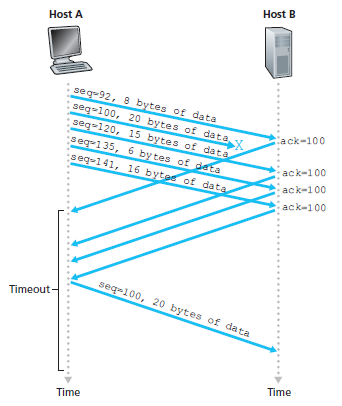
\includegraphics[width=0.9\linewidth]{cap10/fast_retransmit.png}
\end{minipage}\hfill
\begin{minipage}{0.62\linewidth}
\begin{itemize}
  \item Si perde il segmento con numero di sequenza 100.
  \item Ogni volta che B riceve un segmento fuori ordine, rimanda un ACK duplicato (ACK=100).
  \item Al terzo duplicato A considera perso il segmento 100 e lo rispedisce (fast retransmit), senza aspettare il timer.
  \item Quando B riceve finalmente il segmento mancante, invia l'ACK del prossimo segmento atteso secondo la propria
        politica (tipo Go-Back-N o Selective Repeat).
\end{itemize}
\end{minipage}
\caption{Ritrasmissione veloce dopo tre ACK duplicati.}
\end{figure}

\warning{Perché proprio tre duplicati?}{
    Perché non ritrasmettere al primo ACK duplicato? Perché un ACK ``sbagliato'' può arrivare anche per
    motivi diversi da una perdita. Per esempio, se due segmenti arrivano \textbf{scambiati di ordine}, il ricevente
    invia un ACK duplicato (per il primo segmento) prima di accorgersi dello scambio. Aspettare tre duplicati
    evita ritrasmissioni inutili dovute al semplice riordinamento: tre di fila sono difficili da spiegare così, perché
    vuol dire che tre segmenti successivi sono passati mentre quello no. Il numero è un compromesso fissato dalle misure
    più che derivato: tre è il valore su cui si è assestato lo standard.
}

% ══════════════════════════════════════════════════════════════
\section{Go-Back-N o Selective Repeat?}
% ══════════════════════════════════════════════════════════════

\begin{itemize}
    \item \textbf{Come Go-Back-N}: conferme cumulative, nessuna risposta individuale per ciò che arriva in anticipo, un timer
          e due variabili.
    \item \textbf{Diversamente da Go-Back-N}: un timeout ritrasmette un segmento, non tutto ciò che è in sospeso, e
          nemmeno quello se la conferma successiva lo copre.
    \item \textbf{Come Selective Repeat}: il ricevente tiene in un buffer ciò che arriva in anticipo invece di buttarlo.
\end{itemize}

TCP quindi \textbf{non è nessuno dei due}: conferme cumulative sopra un ricevente che conserva, cioè la metà utile di
ciascuno. Un'opzione, la \key{conferma selettiva} (\emph{SACK}), permette al ricevente di nominare i blocchi che sta
tenendo, e porta TCP il resto della strada.

\Needspace{20\baselineskip}
% ══════════════════════════════════════════════════════════════
\section{Riepilogo}
% ══════════════════════════════════════════════════════════════

\riepilogo{
\begin{itemize}
    \item TCP è orientato alla connessione, affidabile, full-duplex, punto-punto e orientato al flusso di byte,
          con buffer di invio e ricezione.
    \item $\text{MSS} + 40 = \text{MTU}$ (in Ethernet MSS tipica 1460 byte).
    \item Header TCP: porte, \textbf{Seq}, \textbf{ACK}, lunghezza, flag (SYN, ACK, FIN, RST, \dots), finestra di
          ricezione, checksum, opzioni.
    \item Seq = numero del primo byte del segmento; ACK = prossimo byte atteso (cumulativo).
    \item $\text{EstimatedRTT} = 0{,}875\cdot\text{Est} + 0{,}125\cdot\text{Sample}$;
          $\text{DevRTT} = 0{,}75\cdot\text{Dev} + 0{,}25\cdot|\text{Sample}-\text{Est}|$;
          $\text{Timeout} = \text{Est} + 4\cdot\text{Dev}$.
    \item Un solo timer, sul segmento più vecchio non confermato; dopo un timeout l'intervallo raddoppia, e i segmenti
          ritrasmessi non si campionano.
    \item \textbf{Fast retransmit}: 3 ACK duplicati $\Rightarrow$ ritrasmissione immediata.
    \item Resta aperto: come i due estremi si accordano sui numeri iniziali, e a che cosa serve la finestra di ricezione
          nell'header.
\end{itemize}
}
